\documentclass[11pt,letterpaper,fleqn]{article}
\usepackage{rotating}
\usepackage{graphicx}
\usepackage{amsfonts,amsmath}
\usepackage{subfigure} % need for subfigures
\usepackage{wrapfig}
\usepackage[margin=1in]{geometry}
\usepackage{cite}
\usepackage{amssymb}
\usepackage[final]{pdfpages}
\usepackage{hyperref,enumitem}
\hypersetup{
colorlinks, citecolor=blue, filecolor=black, linkcolor=blue, urlcolor=blue}
\usepackage{booktabs}
\usepackage{multirow}
\usepackage{siunitx}
\sisetup{group-separator = {,}}
\usepackage{titlesec}
\titlespacing\section{0pt}{6pt plus 4pt minus 2pt}{0pt plus 0pt minus 0pt}
\titlespacing\subsection{0pt}{6pt plus 4pt minus 2pt}{0pt plus 0pt minus 0pt}
\titlespacing\subsubsection{0pt}{6pt plus 4pt minus 2pt}{0pt plus 0pt minus 0pt}
\usepackage{titling} % Allows custom title configuration
\usepackage{fancyhdr} % Needed to define custom headers/footers
\usepackage{lastpage} % Used to determine the number of pages in the document
\usepackage[english]{babel}
\usepackage{blindtext}
%\usepackage{draftwatermark}
%\SetWatermarkText{Draft v0.0}

% Add you own definitions here (file report-defs.sty).
\usepackage{report-defs}

%-------------------------------------------------------------------------------
%   TITLE SECTION
%-------------------------------------------------------------------------------

\date{} % blank out date from fancyhdr

\pretitle{\vspace{-50pt} \begin{flushleft} \fontsize{15}{15} \usefont{OT1}{phv}{b}{n} \selectfont} % Horizontal rule before the title
\title{\large Summary of Blueprint Workshop: \\
\vspace{1pt}
%\color{red}
\LARGE \textit{Analysis Systems R\&D on Scalable Platforms} \\
\color{black} \normalsize
\vspace{10pt}
June 21--22, 2019 \\
New York University \\
Meeting URL: \href{https://indico.cern.ch/event/820946/}{https://indico.cern.ch/event/820946/}
} % Your article title
\posttitle{\par\end{flushleft}\vskip 0.5em} % Whitespace under the title
\preauthor
{
  \begin{flushleft}
    \vspace{-13pt}
    {\normalfont Workshop Organizers:} \\
    \vspace{3pt}
    \large \lineskip 0.5em \usefont{OT1}{phv}{b}{sl} \color{black}} % Author font configuration
    \author{Kyle Cranmer {\normalfont(New York University)}
      \and  Rob Gardner {\normalfont(University of Chicago)}
      \and  Mark Neubauer {\normalfont(University of Illinois at Urbana-Champaign)}
      }
      \postauthor{\par
      \vspace{10pt}
      {\normalfont Summary prepared by:} \\
      \vspace{3pt}
      Mark Neubauer {\normalfont(University of Illinois at Urbana-Champaign)}

\end{flushleft} \vspace{-10pt} \HorRule} % Horizontal rule after the title

\renewcommand{\and}{\\}

%-------------------------------------------------------------------------------

\begin{document}
\maketitle % Print the title
\normalfont

\thispagestyle{firststyle}

\vspace{-45pt}

\section*{Major Goals}
\vspace{3pt}
\begin{itemize}
  \item Review the status of the Analysis Systems (AS) milestones and deliverables.
  \item Develop the Scalable Systems Laboratory (SSL) scope, architecture and plans, using AS R\&D activties as concrete examples.
  \item Develop requirements on SSL to support the AS area, particularly the prototyping, benchmarking and scaling of AS deliverables toward deployment.
  \item Increase the visibility of SSL and AS R\&D beyond IRIS-HEP to facilitate partnerships with organizations that could potentially provide software and computing resources for SSL.
  \item Get informed on latest developments in technologies and methods relevant for SSL and AS.
\end{itemize}

\section*{Key Outcomes}
\vspace{3pt}
\begin{itemize}
  \item Communication of the AS area plans and preliminary requirements to SSL.
  \item Kubernetes as a planned {\it common denominator} for SSL, increasing the capabilities through flexible infrastruture. This idea spawned plans for a multi-site SSL {\it substrate} project that will federate SSL contributions from multiple resource providers, offerring the AS area a flexible platform for service deployment at scales needed to test viability of system designs.
  \item Productive engagement of the AS/SSL team with representatives from NCSA, SDSC, NYU Research Computing, industry \& cloud providers (Google, Redhat), generating action items.
  \item A concrete vision for an SSL that serves not as an innovation space for AS developers, but as a testbed to prototype next generation infrastructure for future HEP computing environments.

\end{itemize}

%-------------------------------------------------------------------------------

\newpage
\thispagestyle{reststyle}

\section{Overview}
Together with the OSG-LHC, the Scalable Systems Laboratory (SSL) is designed to be the primary integration path to deliver the output of IRIS-HEP R\&D activities into the distributed and scientific production infrastructure of the experiments. The aim of this workshop is to further develop the IRIS-HEP SSL concept using specific R\&D examples from the AS area, including  low-latency, query-based data systems and modular, reusable cyberinfrastructure for physics inference and results dissemination. Registered attendees include those from IRIS-HEP (primarily SSL and AS areas), US ATLAS/CMS operations programs, national labs, CERN, supercomputing centers (SDSC, NCSA), university research IT, and industry (RedHat, Google).

The venue for the workshop was the Physics Department at New York University and was hosted by Kyle Cranmer.  The blueprint meeting benefited by its proximity to the IRIS-HEP \href{https://indico.cern.ch/event/822074/}{Analysis Systems Topic Workshop} which immediately proceeded it.

\section{Attendees}
There were 26 \href{https://indico.cern.ch/event/820946/registrations/participants}{registered participants} for workshop, with all but a few attending in person. The workshop attendees were:
Andrew Chien (Chicago),
Andrew Melo (Vanderbilt),
Aravindh Puthiyaparambil (Red Hat),
Benjamin Galewsky (Illinois/NCSA),
Dan S. Katz (Illinois/NCSA),
David Ackerman (NYU),
Edgar Fajardo (SDSC),
Eric Borenstein (NYU),
Gordon Watts (Washington),
Ianna Osborne (Fermilab),
Jim Pivarski (Princeton),
Kyle Cranmer (NYU),
Lincoln Bryant (Chicago),
Lindsey Gray (Fermilab),
Mark Neubauer (Illinois),
Mason Proffitt (Washington),
Matthew Feickert (SMU),
Nils Krumnack (Iowa State),
Ricardo Brito Da Rocha (CERN),
Rob Gardner (Chicago),
Sanjay Arora (Red Hat),
Stephen Fang (Google),
Stratos Efstathiadis (NYU),
Tatiana Polunina (NYU),
Tim Boerner (Illinois/NCSA),
Wei Yang (SLAC)

\section{Goals}
The primary goals of the workshop were to
\begin{itemize}
  \item Review the status of AS milestones and deliverables
  \item Develop the Scalable Systems Laboratory (SSL) scope, architecture and plans, using Analysis Systems (AS) R\&D activties as concrete examples.
  \item Develop requirements on SSL to support the AS area, particularly the prototyping, benchmarking and scaling of AS deliverables toward deployment.
  \item Increase the visibility of SSL and AS R\&D beyond IRIS-HEP to facilitate partnerships with organizations that could potentially provide software and computing resources for SSL.
  \item Get informed on latest developments in technologies and methods relevant for SSL and AS.
\end{itemize}
Significant progress was made towards each of these goals.


\section{Activites}

The meeting was structured as a series of informal presentations which sufficient time for in-depth discussions.  In advance of the meeting we identified some specific objectives to guide discussions:

\begin{itemize}
  \item Collection and curatation of analysis use cases, each with a reference implementation.  What patterns and infrastructure are needed?
  \item Translation of analysis examples into new specifications, providing feedback and iteration.
  \item Development of initial specifications for user-facing interfaces to analysis system components.
  \item Benchmarking of existing analysis components and integrating the benchmarking into SSL.
  \item Development of accelerator-based fitting \& statistical tools (and other relevant components).
  \item Integrating prototypes of AS components into SSL, followed by benchmarking \& assessment.
\end{itemize}

\subsection{Presentations and Discussion}

There were eight presentations chosen to trigger discussion on the main themes and objectives of the workshop.


\subsubsection{The Blueprint Process}
Mark Neubauer (University of Illinois) presented {\it IRIS-HEP Blueprint Concepts and Process} which provided a broad overview of not only the blueprint process but the data and processing challenge to set the context. This was particularly helpful for workshop participants new to computing in HEP and the HL-LHC computing scale.

\subsubsection{The SSL Concept}
Robert Gardner (UChicago) presented {\it Scalable Systems Laboratory (IRIS-HEP) - challenges, opportunities}.  The program of work of the SSL activity was described.  Given the SSL core has less than an FTE of effort, success will depend on leverage efforts from other areas of IRIS-HEP and engaged partners. The high level purpose of the SSL is to provide the Institute and the HL-LHC experiments with scalable platforms needed for development in context, i.e. the {\it path to production}:

\begin{itemize}
  \item Provides access to infrastructure and environments
  \item Organizes software and resources for scalability testing
  \item Does foundational systems R\&D on accelerated services
  \item Provides the integration path to the OSG-LHC production infrastructure
\end{itemize}

The challenges are that it must be a community platform across experiments and institutions; it should support groups/projects with specific organizational membership for access; it must aggregate bespoke resources \& configurations; it must do so in {\it delcarative} fashion such that deployments are reproducible and {\it mobile}; it must provide services to build \& management deployment artifacts; and it must be scalable up and down.

The opportunities presented are that in building out the SSL adhoc collaborations will be formed which cross organizational boundaries; contributions will come from diverse resource providers, broadening participation; new models of infrastructure development will be formed supporting more rapid innocation of new analysis systems; and that artifacts can be redeployed generally will accelerate delivery of R\&D systems to the community for use in production.

It was noted that storage and networking become a big issue for the large data sets we’re dealing with, and so how does the SSL reach relevant scale for feasibility testing?  The possibility of augmenting with cloud resources was discussed (an example of a several million cores provided to an MIT researcher was noted), and comparison costing with on-prem resources.  It was agreed this should always be considered and costs periodically assessed.  Additionally research partnerships where there is mutual interest with public cloud providers should continue to be exploited.   Finally, specifics of the server/instance targets need to be considered, such as memory/core and I/O bandwidth which could pose special challenges and costs.


\subsubsection{Analysis Systems}
Kyle Cranmer (NYU) presented {\it Analysis Systems Perspectives \& Goals}.  The just finished \href{https://indico.cern.ch/event/822074/}{Analysis Systems Topic Workshop} revisited the milestones and deliverables for the rest of IRIS-HEP Year 1 and and Year 2 planning.  It was noted there are AS scalbility milestones in Y2Q1 which imply requirements on SSL readiness,  The goal is to move testing on whatever resources currently in use to an {\it SSL-managed} infrastructure.
This includes prototypes of analysis systems components to be deployed on the SSL (Aug '20).

There were notable adhoc demos of interest to the workshop. First was the REANA/RECAST demo at KubeCon 2018, focusing on real analysis reproducibility, demonstrated that HEP can engage with modern open source tools and communities.  Second was the scalability demo of Higgs rediscovery on Kubernetes (200 GB/s, 70 TB) performed at KubeCon and CloudNativeCon Europe 2019.  There are other examples in our field, e.g. \href{https://www.youtube.com/watch?v=Ye8MlJQumaI}{CERN’s Next Generation Data Analysis Platform with Apache Spark} by Enric Tejedor (CERN) at the Spark+AI Summit Europe in London, October 2018.

A number of systems have or will soon emerge from AS that are candidates for deployment and testing on the SSL.

\begin{itemize}
  \item {\it ServiceX}: Part of DOMA's efforts to develop the intelligent data delivery services (IDDS), the service focuses on reformatting data a the end-stage analysis phase, transforming event data into columnar formats which provide advantages for effciency and Python-based processing frameworks.
  \item {\it Coffea}: A columnar analysis framework being developed at Fermilab. It was noted that soon there are ServiceX + Coffea demonstrators
  \item {\it MADMINER}: Containerized workflows with mix of CPU and GPU/TPU acceleration, toward the integration of simulation, machine learning, and statistical inference to reduce time-to-insight. These workflows are ready for execution on Kubernetes using REANA and identified as primary candidates to exercise analysis systems technologies and infrastructurre for physics.
  \item {\it AMPGEN} \& {\it pyhf}: Tools under development toward fitting-as-a-service. Have resources setup and available for users to upload information (e.g., pyhf JSON) and then the service performs the fit. Saves the user from being required to set things up on their own (services are simple, but not everyone has a nice GPU cluster ready to go).
\end{itemize}

The types of systems the AS team has considered for development and testing were discussed.  These incluced public cloud (speed of startup, additional services), university resources (on-prem costs, data storage), existing grid infrastructure (e.g. the Open Science Grid) which has a dedicated integration team (OSG-LHC) in IRIS-HEP, DOE and NSF leadership class HPC systems.  The importance of having the ability to move service deployments and workloads between these resource categories was noted.
The role of container usage on the grid was discussed, including early applications in distributed training (hyperparameter tuning).  Much existing work can be leveraged here, with previous efforts reported at \href{https://indico.cern.ch/event/708041/}{ACAT 2019}, and talks on machine learning in ATLAS using Docker images.
The possiblity of providing HPC "backends" to REANA, including HPC, was discussed and considered a worthy goal.  An interesting side topic was the emerging market place of resources for machine learning outside the public cloud providers and HPC centers; in particular \href{Vast.ai}{vast.ai} provides a cloud computing,   matchmaking and aggregation service focused on lowering the price of compute-intensive workloads.


\subsubsection{SSL Architectural Principles}
Lincoln Bryant (UChicago) presented {\it SSL patterns: hybrid models, developer support, deployments}.  There are a number of desirable features that have been identified for the SSL.  These include community access - open to all working on software infrastructure in HEP - which can be implemented with federation tools based on CI-Logon, for example, providing a single sign-on capability; a lightweight group (project) management system; infrastructure itself should be {\it composable and reusable}; being able to accommodate/aggregate a diverse resource pool and user community; a container-based service orchestration on dedicated resources; \href{http://www.virtualclusters.org/}{VC3}-like technology to connect to HPC/HTC resources for batch scale-out; facilitate integration of commercial cloud resources when needed;

Regarding declarative \& reproducible deployments, the goal is to have infrastructure built under the SSL to be easily reusable and deployable to other sites. The
declarative nature of Kubernetes is a good fit and gets us a long way down that road.

SSL itself should not become a production center; rather it should serve as an incubator for projects which then {\it graduate} to become full-fledged infrastructures that run on production resources. Services to build \& manage artifacts, tools that provide SSL to be scaled up and then back down are part of reducing cognitive load for developers and deployers.

The SSL team is currently using Google Cloud Platform (its Kubernetes Engine) to test ServiceX deployment; this will soon be pulled that off into in-house resources.

From the university point of view, groups which would like to reproduce AS systems locally should have resources to have simple versions of what they need to provide, e.g., a base Kubernetes cluster, a functional REANA instance, as a start.  From campus IT/research technology point of view, easy to deploy systems offer the ability to make a compelling case to the Dean/Provost that they are providing resources that enable good science.


Suggested were some light-weight mechanisms for discovery of resources.   The value of reporting and showing science that is happening on the contributed resources to incentivize resource providers at the universities was noted.  Capturing success stories, so university community understands how they can benefit from investments to shared campus resources, including staff, were noted.  Having a dashboard may help communicate the contributions.  This would be important for products that can be used outside HEP, giving them higher visibility.

There were questions as to whether the SSL provisioning method, dashboard panels, and other tools developed to materialize and manage the service infrasructure would be open sourced and productized?  These were interesting possibilities and would depend on the level of effort and other priorities.


\subsubsection{Experience with Google Cloud Platform}

Lukas Heinrich (CERN) presented {\it Ecosystems I: Google Cloud Platform}.  The KubeCon 2019 keynote \href{https://sched.co/MRyv}{Reperforming a Nobel Prize Discovery on Kubernetes} was illustrative of the power and flexibility of Kubernetes and its relevance the HEP computing.  The CMS open data sample (70 TB, 25000 files) was reprocess on stage using legacy software from the CMS scientific software stack using Kubernetes at a large scale.  The main lessons learned were that the Google Network can serve extreme data rates into compute nodes (2 Gbps/core) once handled appropriately. Incoming data could be staged using Google tools but disks that can handle the required rates are scarce (local SSD drives).  A write-to-memory scheme was therefore developed. At highly parallel workloads, scheduling become very important and these systems are still undeveloped in Kubernetes.

\subsubsection{Easing Kubernetes Deployment}

Sanjay Arora (RedHat) presented {\it Ecosystems II: RedHat OpenShift}.  \href{https://www.openshift.com/}{OpenShift} is distribution of Kubernetes that makes on-prem clusters easier to deploy and maintain.  The model is similar to RedHat release of Linux, and there is an open source equivalent to CentOS for OpenShift: \href{https://www.okd.io/}{OKD}.  If Kubernetes is to play a central role in a re-engineered WLCG computing infrastructure, its distribution and management could benefit from solutions such as these and similar.


%\subsubsection{Perspectives from University Resource Providers}
%David Ackerman (CIO, NYU) presented {\it Resource providers: university perspectives}.


\subsubsection{Accelerated Systems}

Andrew Chien (UChicago) presented {\it Accelerated Systems and Optimization}.  System scalability research offers an opportunity to optimize use of resources in specific areas in an end-to-end computing system.   In a local database, it is about query optimization with predicates and filters; by exploiting selectivity one can increase the scalability and performance of a system. In a public cloud context, services such as \href{https://aws.amazon.com/blogs/aws/s3-glacier-select/}{AWS S3 Select} offer the ability to accelerate services through partial selection of objects before delivery to clients.  Opportunities in HEP include (optionally hardware) filtering in strategic locations to reduce traffic on the wide area network.  Previous findings on studies of data transformation with recoding accelerators, with programmable accelerators allowing the right representation choice (and format) performed in the {\it right place} have potential for cheaper computation, less data movement and higher performance.

Throughout the presentation a number of {\it dimensions of benefit} involving system optimization choices with acceleration were identified:

\begin{itemize}
  \item Reduction in parsing \& filtering costs (through acceleration)
  \item Performance through more aggressive query optimization
  \item Representation of encoding in Query Execution Plan
  \item Beyond tuple to block/transpose, special recoding (ex. ML inference and analysis for systems), etc.
  \item Expose new optimizations, eliminate transformation overhead
  \item Reduces the CPU load, offloaded computation, reduce total data processed
  \item Shift of Filtering computation to Storage node
  \item Reduces Data Center network load
\end{itemize}


\subsection{Afternoon Discussion}

In thinking of concrete progress for AS-SSL activities, \href{http://www.reanahub.io/}{REANA} was identified as a likely good first deployment target for the SSL. In addition, ServiceX as deployed on Google Cloud Platform via Helm would make it an interesting use case if the SSL API is Kubernetes.

We discussed an REANA deployed on an SSL cluster provisioned with OpenShift. Success of the deployment would be to have two independent sets of people deploy. Templated python scripts, HELM charts, and YAML would be the ingredients.  What would be needed from the SSL?

\begin{itemize}
  \item Storage
  \item Internet ingress
  \item Load balancing
  \item Pod capacity
\end{itemize}

Other questions arose: {\it Is there one SSL (as a service) or a standard?} As a pattern, we'd like not to have a site administrator having to follow notes off a twiki to stand up Kubernetes. We’d like the admin to connect their nodes to an SSL console and everything is automatically deployed. The process to join must be lightweight. If one observes a deployed pattern, they should be able to deploy the pattern to a local environment.

If you use SSL then you should at least publish deployment instructions so others can reproduce it. An R\&D Hybrid Cloud provider. Try to make the substrate as compatible as possible with CERN-IT and FermiLab.

Question: {\it if a federated set of Kubernetes clusters is the substrated approach for SSL, do we lose anything there? Are there any blockers to this approach for the AS R\&D plans on SSL?}  The answer for AS was that there does not seem to be, but maybe HPC integration would need further consideration. For scaling test, federating SSL clusters will be desirable.

{\bf Metric data} would be useful to have from SSL.  Dashboards and retention of results, the ability to mine metadata indexed by ElasticSearch, use of Kubernetes monitors such as Prometheus would provide some of this.  Developing the complete suite for logging and metrics collection is out of scope of SSL, but maybe provide a few standard tools and a repository to collect notes on best practice.

There were comments that not everyone in our group knows how to build a Helm chart, the (current) defacto standard for Kubernetes deployments. While that is true, often the stuff we are all working on is going to fit into a Helm chart eventually - so there is something to be said for being able to at least use it. Docker/desktop can run kubernetes and I don’t know how hard it is to make a flexible chart that can scale from a single node cluster to many, but this means that the person working on the component can basically run it in the environment they will eventually have to run in. Generally it was agreed the burden would be to the R\&D areas to define the metrics and guide SSL on what data to retain.

We discussed SSL {\bf service Level agreements} between research teams and the SSL; their role and utility for setting developer and resource provider expectations.  Some ideas included agreement to publish deployment artifacts; ability to request time and scheduling for scalability tests;  agreement the needed information is agreed upon before devoting significant resources.

Opportunities \& planning for resources was discussed.  Should there be regions of the SSL where clusters nearby are logically group or technically joined via a federation or mesh software. It was agreed that successful contributins would rely on tools that allow operators the ability to re-create SSL environments at another location.  Specific initial sites discussed included:
\begin{itemize}
  \item NCSA: the ISL (Integrated Systems Lab), the Openstack cluster, Blue Waters (a short term allocation), the Illinois Campus Cluster (opportunistic use of GPUs), and an NSF MRI Deep Learning research platform
  \item Redhat (Openshift) - there is the Massachusetts Open Cloud
  \item CERN
  \item NYU
  \item Fermilab
  \item BNL
  \item SDSC and the Pacific Research Platform
\end{itemize}

\subsection{Day 2 Breakout Session}
On the second day, participants broke into two (roughly equal) groups for more detailed discussion and development of the key workshop outcomes and action items. One group examined specific issues related requirements from the Year 2 plan for AS. The second group assembled to discuss topics around SSL infrastructure and to identify an impactful path moving forward. The assignment of which participants were in which group was voluntary based on interests of each participant.

\subsubsection{Analysis Systems Breakout}

The AS breakout session was lead by Kyle Cranmer who began with a presentation of the milestones, as shown in Figure~\ref{fig:AS_milestones}.
\begin{figure}
  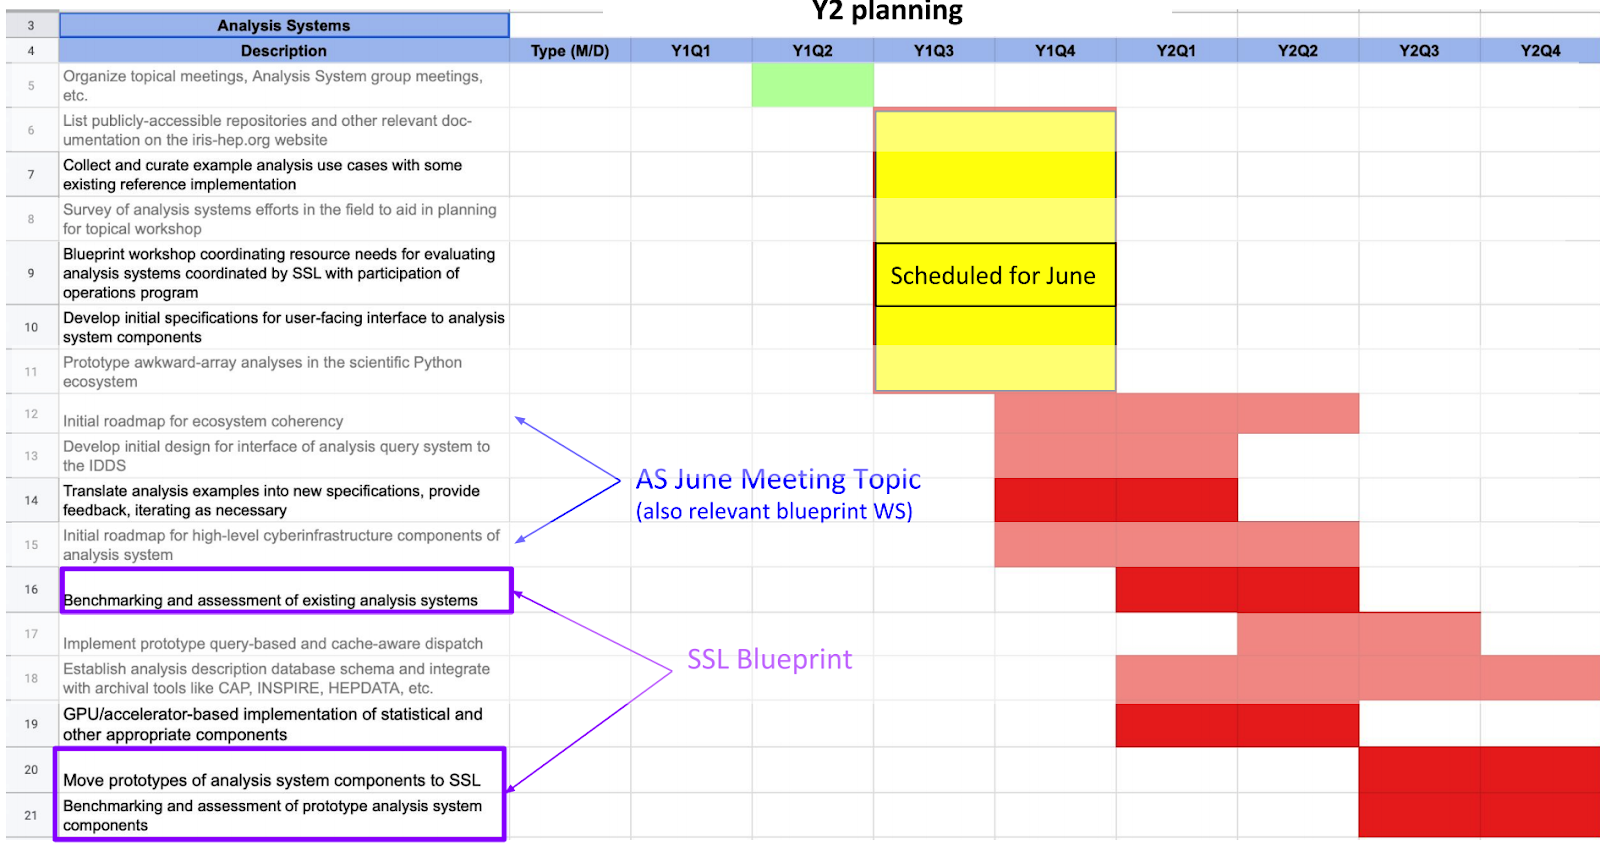
\includegraphics[width=\linewidth]{figures/as_milestones.png}
  \caption{Annotated snapshot of the AS milestones presented in the AS breakout session on Day 2 of the workshop.}
  \label{fig:AS_milestones}
\end{figure}
The following discussion focused on answering the following question: {\it What SSL cyberinfrastructure is required for AS success?}. Key elements that were put forward during the discussion included:
\begin{itemize}
  \item {\it Lowering barriers for participation in analysis systems} that are currently under development. This includes clear and thorough documentation, particularly the devalopment and maintenance of workuing examples
  \item {\it Empowering small groups with limited physical infrastructure and personnel to contribute meaningfully to data analysis}. There are growing concerns within the HEP communitiy that it is becoming increasingly difficult for single-PI groups to make a strong impact to physics papers on the large experiments. This issue is on the radar screen of the agencies as well and touches on challenges around diversity and outreach. It was pointed out that one way to address this challenge is to streamline the process of onboarding and transfer ("forward evolution") of analyses. As an example, RECAST represented a new style of doing analysis which CERN cloud servies facilitated. Similarly, there are \href{https://gitlab.cern.ch/aml/containers/docker}{ATLAS base Docker images} for machine learning. If SSL can provide these types of services quickly it would move forward critically-needed developments in this area.
  \item {\it Establishing mechanisms for SSL to coordinate with campus IT efforts to replicate working environments} For example, NYU and k8 research clusters were proposed to test this paradigm. This activity could also inform the future evolution of the Tier-2s.
  \item {\it SSL as a matchmaker and hub for relationships} of analyzers and developers.
  \item {\it BinderHub connected to SSL authentication} as one of the capabilities in the SSL service catalogue. A
  \href{https://mybinder.org/}{Binder} example is the \href{https://mybinder.org/v2/gh/diana-hep/pyhf/master?filepath=docs%2Fexamples%2Fnotebooks%2Fbinderexample%2FStatisticalAnalysis.ipynb}{pyhf example stat analysis}. 

\end{itemize}

\subsubsection{SSL Infrastructure Breakout}




\section{Action Items}
The following action items were identified:
\begin{enumerate}
  \item Deploy an AS validator application on the initial SSL cluster at UChicago
  \item Identification of institutes with interest in building the SSL substrate
  \item Organization of regular SSL technical meetings
\end{enumerate}

\section{Feedback from Attendees}
\begin{itemize}
  \item Some participants expressed interest in having more preparatory documents available in advance of the meeting.  This was seen as particularly important for participants new to high energy physics computing or IRIS-HEP, including potential industry partners.
  \item In the preceeding Analysis Systems Topical Workshop, much discussion focused on establishing community development patterns and management infrastructure more in aligned with best practices found in professsional engineering settings.
  \item The planning for the meeting should have begun sooner to ensure the needed representation from participants and subject focus.
\end{itemize}

\section{Summary}
\blindtext[2]

\appendix
\newpage
\section{Revision History}

\vspace{8pt}
\begin{itemize}
  \item Version 0.0
  \vspace{-5pt}
  \begin{itemize}
    \item Initial version
  \end{itemize}
  \item Version 0.1
  \vspace{-5pt}
  \begin{itemize}
    \item Version for IRIS-HEP Executive Board review
  \end{itemize}
\end{itemize}

\end{document}
